% ANÁLISIS

\section{Toma de requisitos}

En el desarrollo de esta aplicación la toma de requisitos se hizo mediante reuniones con el tutor del proyecto,
que realizaba el papel de cliente potencial de la misma. Después de varias reuniones se obtuvo el listado de requisitos
que se muestra en las siguientes secciones:


\subsection{Requisitos de interfaces externas}

En este apartado se van a describir los requisitos de conexión entre el software y el hardware, así como la interfaz
del usuario.\\

De la interfaz entre el software y el hardware se encarga la librería SDL, mediante el wrapper pygame --- y por encima
la capa que añade Gloss--- que, al ser un sistema preestablecido, no será necesario analizarlo ni diseñarlo,
simplemente haremos uso de él.\\

Así que pasamos a definir el interfaz entre el videojuego y el usuario. Todas las ventanas de la aplicación podrán
ser mostradas a pantalla completa o en formato de ventana con una resolución de 800 por 600 píxeles. A
continuación se definen las distintas ventanas con las que el usuario se puede encontrar:

\begin{description}
    \item[Ventana de introducción] Esta primera ventana mostrará únicamente el logotipo de Dominous, situando al usuario
            en contexto para iniciarlo en la ejecución del programa
    \item[Ventana del menú principal] La ventana del menú principal muestra el menú de inicio de Dominous, en el que
            el usuario podrá elegir entre las opciones más generales del juego, entre las que se encuentran:
            \begin{itemize}
                \item Partida clásica
                \item Laboratorio
                \item Opciones
                \item Tutorial
                \item Salir
            \end{itemize}
            Este menú y los siguientes que se describan serán completamente manejados por el ratón y bastará
            un clic encima de una opción para acceder a ella.
    \item[Ventana de selección de personaje] Esta ventana mostrará una interfaz que permite al usuario elegir los
            diferentes participantes que se enfrentarán en la siguiente partida. En caso del modo laboratorio
            se elegirán los cuatro jugadores, y en caso de partida clásica serán tres jugadores controlados por
            el ordenador más el jugador humano.
    \item[Ventana de partida] Esta será la ventana principal de todo el juego. Mostrará una partida de dominó
            de dos equipos, el tablero e información de la partida, e irá actualizando el tablero según se vaya
            desarrollando la misma partida. Mediante la pulsación de la tecla ESC o clic sobre el botón menú se
            desplegará el menú interno de la partida, que permitirá abandonarla a pesar de no haberse terminado
            la partida actual.
    \item[Ventana de laboratorio] La ventana de laboratorio proporciona una interfaz para que el usuario de la
            aplicación pueda generar un conjunto elevado de partidas entre dos equipos definidos, con la idea
            de poder decidir qué pareja presenta las mejores características de Inteligencia Artificial.
    \item[Ventana del modo tutorial] Por último la ventana del modo tutorial mostrará al usuario información sobre
            el juego del dóminó mediante un conjunto de presentaciones, para que el mismo usuario pueda aprender
            más sobre el mundo del dominó sin necesidad de salir de la aplicación.
\end{description}


\subsection{Requisitos funcionales}

Los requisitos funcionales que el sistema debe ofrecer al usuario son los siguientes:
\begin{itemize}
    \item Poder jugar una partida de dominó con tres jugadores más controlados por el ordenador.
    \item Enfrentar a dos parejas de jugadores controlados por ordenador, haciendo que jueguen un gran número
            de partidas seguidas en modo automático (esto es, sin visualizar la partida que se desarrolla y
            mostrando únicamente las victorias), con la finalidad de poder decidir qué pareja posee una
            inteligencia artificial más avanzada.
    \item Acceder al modo tutorial, para realizar un aprendizaje de las normas, técnicas y usos del dominó.
    \item Cambiar el tipo de juego para que cuatro jugadores manejados por la máquina puedan desarrollar una
            partida en modo visual.
    \item Seleccionar otro tema gráfico para que, tanto fichas como tablero como otros elementos gráficos, cambien
            a gusto del usuario, eligiendo entre cierto abanico de temas.
    \item Cambiar de modo ventana a modo pantalla completa.
\end{itemize}


\subsection{Requisitos de rendimiento}

El rendimiento de la aplicación debe ser tal que permita un desempeño agradable de la partida. Este requisito
hace referencia principalmente a los siguientes asuntos:
\begin{itemize}
    \item El sistema de inteligencia artificial debe ser lo suficientemente ágil y estar ajustado y
            perfeccionado para que los tiempos empleados en cálculos de toma de decisiones no ralenticen
            la partida. Se cuenta como asunto el que, en el desarrollo de una partida de dominó, los tiempos de
            espera también se interpretan, por lo que debemos realizar los cálculos dentro de un cierto
            margen de tiempo.
    \item Por otro lado, el motor gráfico debe estar optimizado para que el usuario no aprecie movimientos
            bruscos a la hora de manejar la aplicación. No olvidemos que estamos desarrollando un videojuego,
            así que el programa debe mostrar cierta agilidad a la hora de realizar movimientos y transiciones
            entre los diferentes estados de la partida, incluyendo menús, fichas, o asuntos relativos a la
            interfaz, como puede ser el arrastrar una ficha a su lugar correspondiente.
\end{itemize}

Es importante recordar en todo momento que estamos desarrollando una aplicación en tiempo real, por lo que
debe primar la velocidad sobre otros factores como el consumo de memoria principal.


\subsection{Restricciones de diseño}
Como bien comentábamos en el punto anterior, a la hora de realizar el diseño de la aplicación tienen que
primar los tiempos de respuesta sobre el consumo de recursos de la memoria principal o secundaria. Esta
es la principal restricción que tendrá el diseño de nuestra aplicación.\\

Los videojuegos están pensados para ejecutarse como aplicación principal, no para compartir recurssos
con otros programas; por esta razón se permite que consuman muchos recursos.


\subsection{Requisitos del sistema software}

La aplicación debe cumplir con los siguientes requisitos de sistema:
\begin{itemize}
    \item La aplicación debe ejecutarse de forma multiplafatorma, incluyendo como mínimo los sistemas operativos:
        \begin{itemize}
            \item En Microsoft Windows --- Realizándose las pruebas en la versión Windows 7 con las últimas actualizaciones
            \item En sistemas GNU/Linux --- Utilizando la distribución Ubuntu en su versión 10.04 con su instalación
                    por defecto y con todas las actualizaciones del sistema.
        \end{itemize}
    \item El código de la aplicación no debe ser dependiente del sistema operativo en el que se desarrolle la aplicación,
            y debe ser un código mantenible y fácilmente ampliable para futuras mejoras y versiones.
\end{itemize}

\section{Modelo de casos de uso}

Para describir los comportamientos que tendrá el sistema, utilizaremos el lenguaje guaje de modelado de sistemas UML;
éste representa los requisitos funcionales de todo el sistema, centrándose en qué hace pero no en cómo lo hace.\\

A continuación describimos uno por uno cada caso de uso.

\subsection{Diagrama de casos de uso}

Como primer paso, debemos mostrar el diagrama de casos de uso que representa la funcionalidad completa de la aplicación.
El esquema utilizado es el siguiente:
\begin{enumerate}
    \item Identificar los usuarios del sistema y sus posibles roles.
    \item Para cada rol definido, identificar todas las formas que tiene de interactuar con el sistema. En el caso
            de Dominous, existe un único rol de acceso a la aplicación, por lo que la especificación de usuario
            será única.
    \item Crear todos los casos de uso para poder describir los objetivos que se desean cumplir.
    \item Estructurar y definir esos casos de uso.
\end{enumerate}

\begin{figure}[h]
  \label{diagrama-casos-uso}
  \begin{center}
    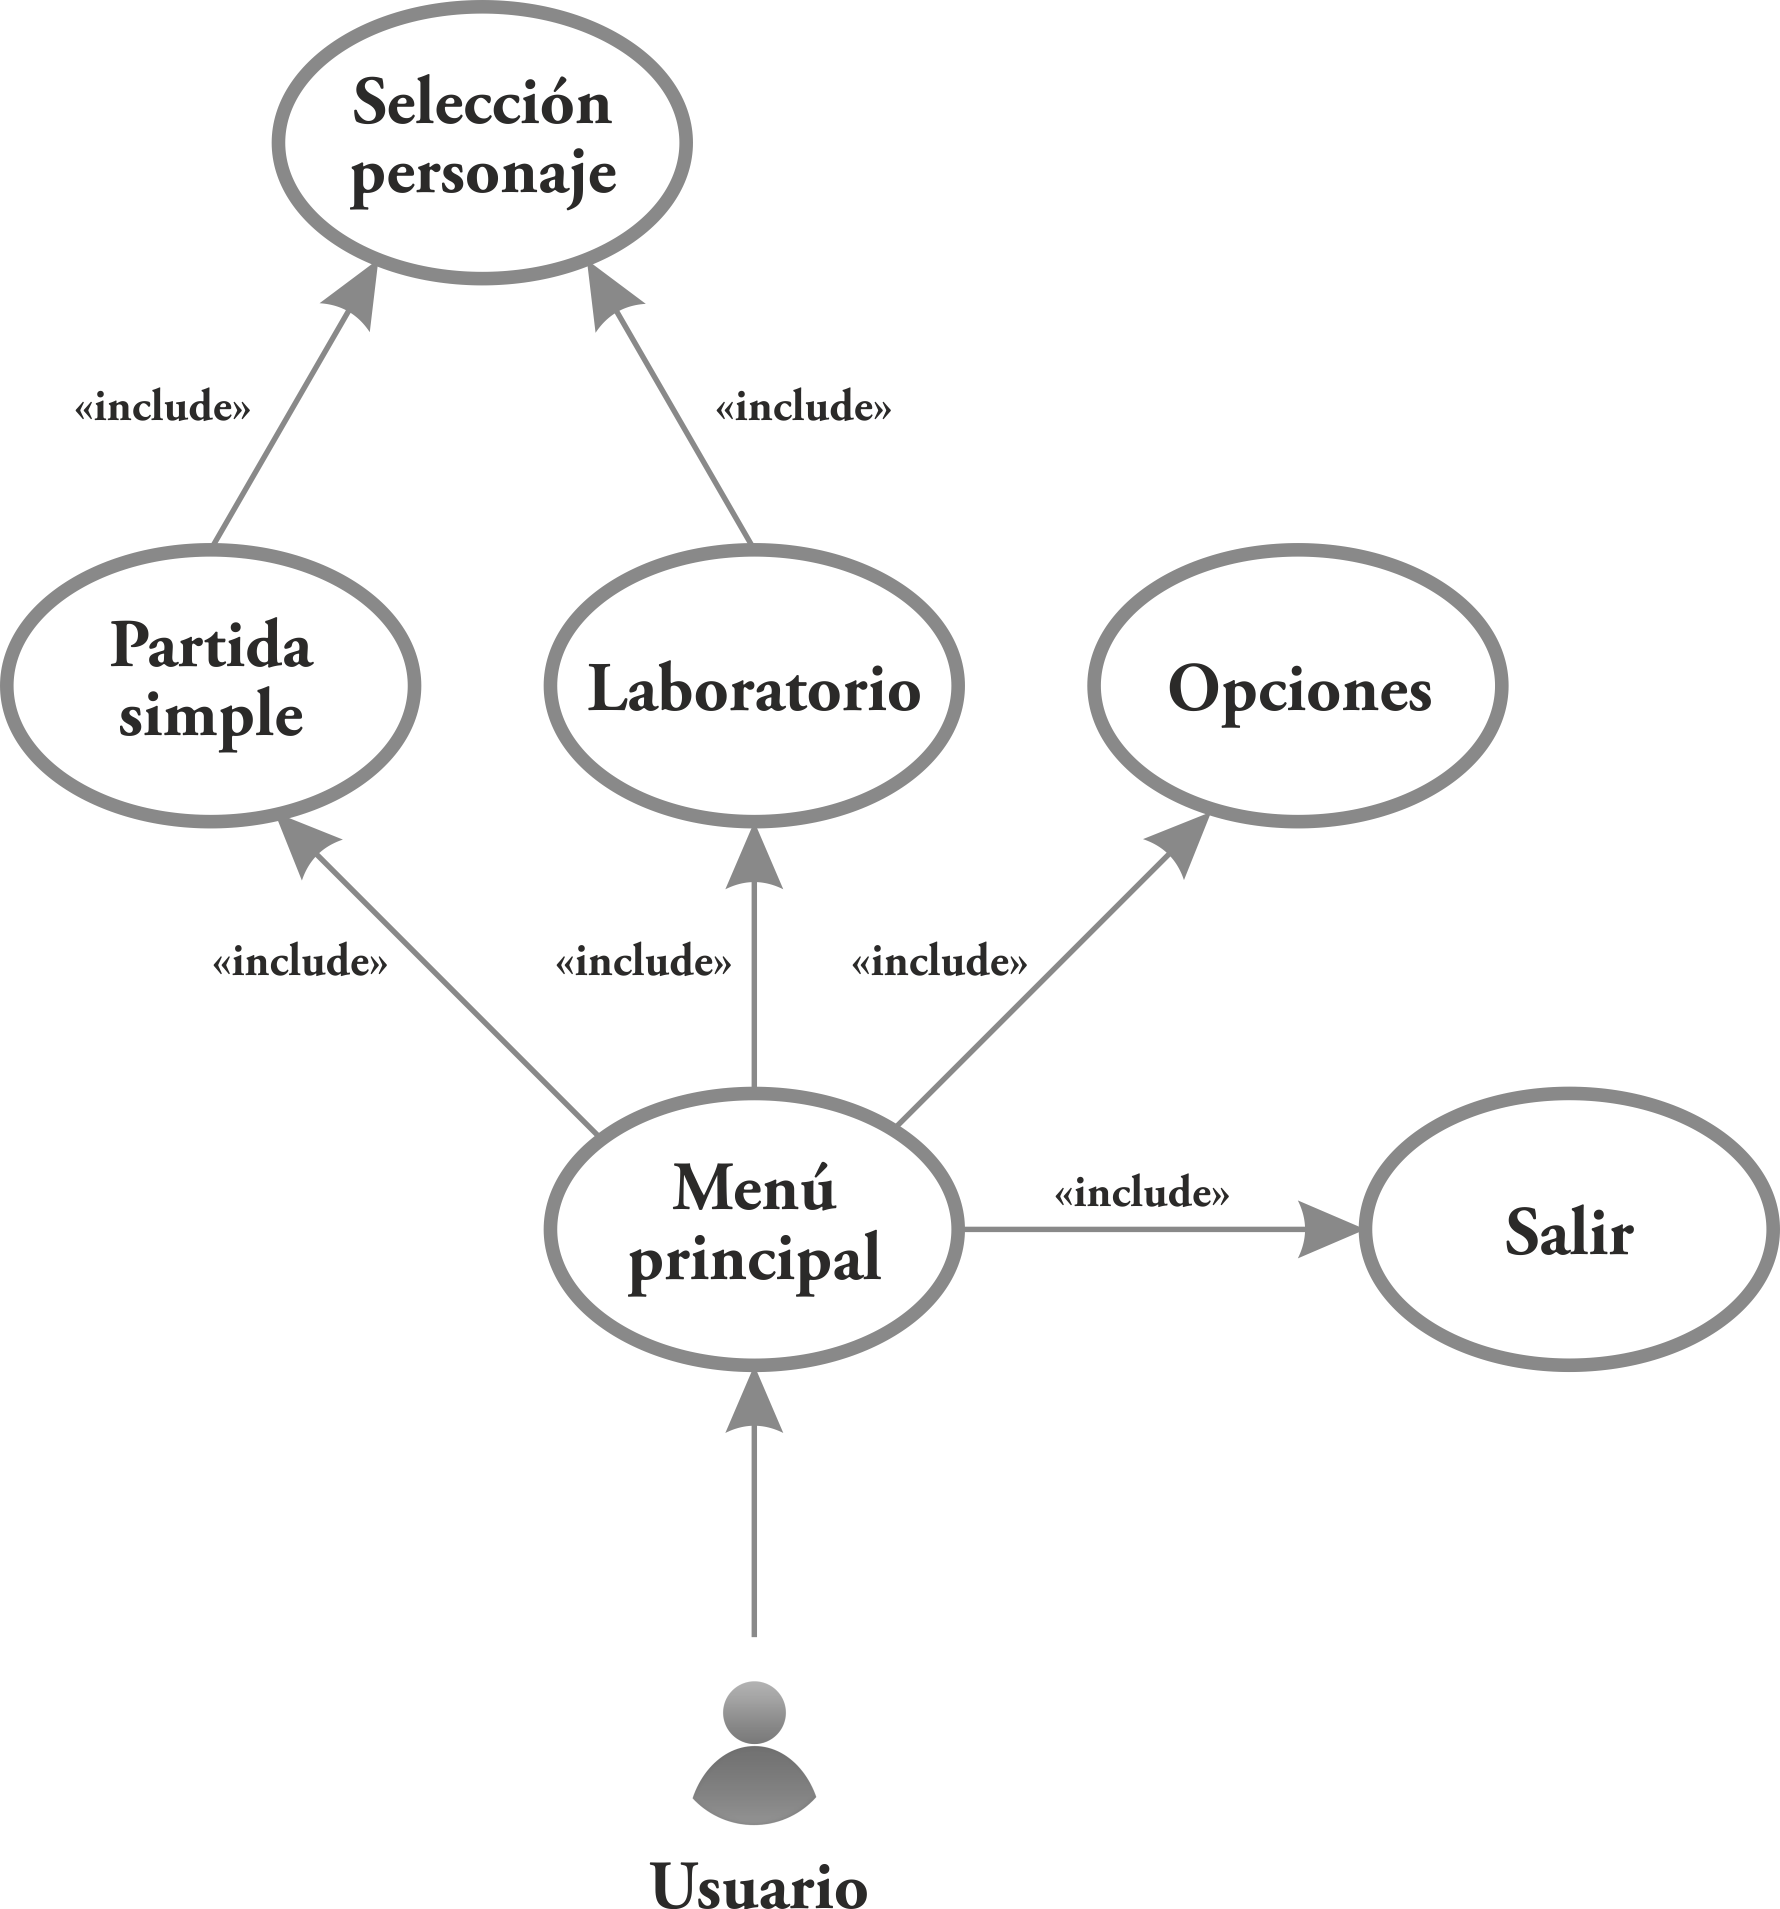
\includegraphics[scale=0.7]{diagrama_casos_de_uso.png}
  \end{center}
  \caption{Diagrama de casos de uso del sistema}
\end{figure}


\subsection{Descripción de los casos de uso}

A continuación pasamos a la descripción de los casos de uso. Para ello se va a utilizar una notación formal
usando plantillas, con la intención y finalidad de que este texto sea legible y comprensible por
un usuario que no sea experto.

\subsubsection{Caso de uso: Menú principal}

\begin{description}
    \item[Caso de uso] Menú principal
    \item[Descripción] Se muestra el menú principal de la aplicación, desde donde es posible acceder a los
        diferentes modos de juego y a las opciones.
    \item[Actores] Usuario
    \item[Precondiciones] Ninguna
    \item[Postcondiciones] Ninguna
    \item[Escenario principal] $\quad$
        \begin{enumerate}
            \item El sistema muestra el menú principal del juego en la pantalla
            \item El usuario selecciona el modo \textbf{partida simple}
            \item El sistema inicia el modo de elección de jugadores
        \end{enumerate}
    \item[Extensiones --- flujo alternativo] $\quad$
        \begin{description}
            \item[*a ] El usuario cierra la ventana de la aplicación y sale de la aplicación
            \item[2a ] El usuario pulsa sobre el botón de laboratorio, dirigiéndose a ese apartado de la aplicación
            \item[2b ] El usuario pulsa el botón de tutorial, dirigiéndose a ese apartado de la aplicación
            \item[2c ] El usuario pulsa sobre las opciones, dirigiéndose a ese apartado de la aplicación
            \item[2d ] El usuario pulsa sobre el botón de salir, cerrándose la aplicación
        \end{description}
   
\end{description}

\subsubsection{Caso de uso: Salir}

\begin{description}
    \item[Caso de uso] Salir.
    \item[Descripción] Primeramente se muestra la pantalla de información de la aplicación --- con más datos
            sobre desarrolladores, licencias y cualquier otra información que pueda resultar de interés para
            el usuario.
    \item[Actores] Usuario.
    \item[Precondiciones] Ninguna.
    \item[Postcondiciones] Se sale de la aplicación.
    \item[Escenario principal] $\quad$
        \begin{enumerate}
            \item El sistema muestra la pantalla de información.
            \item El usuario pulsa sobre cualquier lugar de la aplicación.
            \item La aplicación se cierra.
        \end{enumerate}
    \item[Extensiones --- flujo alternativo] $\quad$
        \begin{description}
            \item[*a ] El usuario cierra la ventana de la aplicación y sale de la aplicación.
        \end{description}
\end{description}
 

\subsubsection{Caso de uso: Partida simple}

\begin{description}
    \item[Caso de uso] Partida simple.
    \item[Descripción] El usuario pulsa el botón partida simple con la intención de comenzar una partida
            de dominó con las opciones por defecto, esto es, jugando por parejas con tres jugadores más
            controlados por el ordenador. El usuario selecciona su pareja de equipo y sus dos adversarios, y
            da comienzo la partida
    \item[Actores] Usuario.
    \item[Precondiciones] Ninguna.
    \item[Postcondiciones] Se jugará una partida de \textbf{Dominous}
    \item[Escenario principal] $\quad$
        \begin{enumerate}
            \item El usuario desea jugar una partida.
            \item El usuario selecciona la opción de menú \textbf{partida simple}.
            \item \texttt{include} \textsc{selección de jugadores}.
            \item El sistema inicializa y muestra la partida actual por pantalla
            \item Por cada mano que se desarrolle:
                \begin{enumerate}
                    \item El usuario y el sistema interactúan durante la partida.
                    \item El sistema muestra quién ha ganado la mano.
                \end{enumerate}
            \item El sistema muestra quién ha ganado al final de la partida.
            \item El sistema cierra la partida y muestra de nuevo el menú principal.
        \end{enumerate}
    \item[Extensiones --- flujo alternativo] $\quad$
        \begin{description}
            \item[*a ] El usuario cierra la ventana de la aplicación y sale de la aplicación.
            \item[2a ] El usuario pulsa sobre cualquier otra opción del menú que no sea la de realizar una
                    partida simple --- se rompe el flujo y se redirige al usuario a la opción elegida. 
            \item[5a ] El usuario pulsa el botón de menú y pulsa en salir de la partida. Se termina la partida
                    actual y se vuelve al menú principal.
        \end{description}
\end{description}

\subsubsection{Caso de uso: Laboratorio}

\begin{description}
    \item[Caso de uso] Laboratorio
    \item[Descripción] El usuario desea realizar pruebas y análisis sobre las diferentes habilidades de cada jugador
            controlado por la Inteligencia Artificial del programa, enfrentando a dos equipos de jugadores a un alto
            número de partidas, y calculando el mejor equipo según el número de victorias alcanzadas.
    \item[Actores] Usuario.
    \item[Precondiciones] Ninguna.
    \item[Postcondiciones] Se realizará una competición a 100 partidas, cada partida jugada a 200 puntos, enfrentando
            a las dos parejas de jugadores seleccionados previamente.
    \item[Escenario principal] $\quad$
        \begin{enumerate}
            \item El usuario desea acceder al modo laboratorio.
            \item El usuario selecciona la opción de menú \textbf{laboratorio}.
            \item \texttt{include} \textsc{selección de jugadores}.
            \item El sistema comienza con los enfrentamientos entre ambas parejas
            \item El sistema finaliza los enfrentamientos y destaca al equipo ganador
            \item El sistema cierra el modo laboratorio y muestra de nuevo el menú principal.
        \end{enumerate}
    \item[Extensiones --- flujo alternativo] $\quad$
        \begin{description}
            \item[*a ] El usuario cierra la ventana de la aplicación y sale de la aplicación.
            \item[*b ] El usuario pulsa el botón de salir del modo laboratorio y se vuelve al menú principal.
            \item[2a ] El usuario pulsa sobre cualquier otra opción del menú que no sea la de realizar una
                    partida simple --- se rompe el flujo y se redirige al usuario a la opción elegida.
            \item[4a ] El usuario pulsa el botón de pausa --- se realiza una pausa en el desarrollo de las
                    partidas, hasta el momento en el que el usuario vuelve a pulsar el botón de pausa y se
                    reanudan los enfrentamientos
            \item[4b ] El usuario pulsa el botón de reiniciar --- se resetean a cero los contadores de partidas,
                    puntos y cualquier otra estadística sobre la que se realice el conteo, y se comienza a
                    desarrollar de nuevo un nuevo conjunto de enfrentamientos.
            \item[6a ] El usuario pulsa el botón de salir del modo laboratorio y se vuelve al menú principal.
        \end{description}
\end{description}

\subsubsection{Caso de uso: Opciones}

\begin{description}
    \item[Caso de uso] Opciones
    \item[Descripción] El usuario decide cambiar alguna elemento de la configuración con la que se desarrollan
            las partidas y que modifican el comportamiento transversal de la aplicación.
    \item[Actores] Usuario.
    \item[Precondiciones] Ninguna.
    \item[Postcondiciones] Se cambian las opciones que se desean modificar por parte del usuario, y se vuelve
            de nuevo al menú principal.
    \item[Escenario principal] $\quad$
        \begin{enumerate}
            \item El usuario desea acceder y cambiar las opciones del juego.
            \item El usuario selecciona la opción de menú \textbf{opciones}.
            \item El sistema muestra todas las opciones.
            \item El usuario pulsa en volver.
            \item El sistema guarda en la configuración general del juego las opciones seleccionadas, para
                    que en posteriores ejecuciones se mantengan las mismas opciones previamente seleccionadas.
            \item El sistema muestra de nuevo el menú principal.
        \end{enumerate}
    \item[Extensiones --- flujo alternativo] $\quad$
        \begin{description}
            \item[*a ] El usuario cierra la ventana de la aplicación y sale de la aplicación.
            \item[*b ] El usuario pulsa el botón volver y se retorna al menú principal.
            \item[2a ] El usuario pulsa sobre cualquier otra opción del menú que no sea la de realizar una
                    partida simple --- se rompe el flujo y se redirige al usuario a la opción elegida.
            \item[3a ] El usuario pulsa en \textbf{modo de juego} --- el sistema va rotando entre las diferentes
                    opciones de juego, que son dos: \textbf{modo de juego un jugador} (el jugador humano participa
                    de la partida) y \textbf{modo de juego solo computadora} (todos los jugadores participantes
                    estarán controlados por la máquina).
            \item[3b ] El usuario pulsa en \textbf{tema gráfico} --- el sistema va rotando entre los distintos
                    temas gráficos que están instalados en la aplicación, y que más tarde cambiarán el aspecto
                    visual de la partida.
            \item[3c ] El usuario pulsa en \textbf{velocidad de juego} --- el sistema permite elegir entre tres
                    tipos de velocidades para la partida: \textbf{velocidad normal}, en el que la partida
                    transcurre a una velocidad pausada y cómoda, \textbf{velocidad rápida}, en el que los jugadores
                    manejados por la máquina colocan las fichas sin realizar pausas para pensar, y \textbf{velocidad
                    extra rápida}, en el que, además de no realizar pausa, las fichas se mueven cuatro veces
                    más rápido de la velocidad normal de juego.
            \item[3d ] El usuario pulsa en \textbf{modo ventana} --- El sistema permite cambiar entre dos modos
                    de visualización del juego: \textbf{modo ventana}, en el que la aplicación se muestra dentro de
                    una ventana controlada por el gestor de ventanas nativo del sistema, y el \textbf{modo pantalla
                    completa}, donde la acción ocupa toda la pantalla activa del usuario.
        \end{description}
\end{description}

\subsubsection{Caso de uso: Selección de personaje}

\begin{description}
    \item[Caso de uso] Selección de personaje.
    \item[Descripción] El usuario desea seleccionar los jugadores que participarán en el siguiente juego
            a desarrollar, ya sea \textbf{partida simple} o modo \textbf{laboratorio}.
    \item[Actores] Usuario.
    \item[Precondiciones] El usuario ha pulsado previamente una de estas dos opciones del menú principal:
            \textbf{partida simple} o modo \textbf{laboratorio}.
    \item[Postcondiciones] Se guardará en configuración los jugadores seleccionados por el usuario para el
            posterior desarrollo del juego.
    \item[Escenario principal] $\quad$
        \begin{enumerate}
            \item El usuario debe seleccionar los personajes que participarán en el juego
            \item El sistema muestra los jugadores actuales.
            \item El usuario selecciona los personajes que jugarán la partida o partidas siguientes.
            \item El usuario está satisfecho con su elección y pulsa el botón de jugar.
            \item El sistema guarda la información de los jugadores seleccionados.
            \item El sistema pasa al siguiente paso, que puede ser \textbf{partida simple} o modo
                    \textbf{laboratorio}, dependiendo del estado de la precondición.
        \end{enumerate}
    \item[Extensiones --- flujo alternativo] $\quad$
        \begin{description}
            \item[*a ] El usuario cierra la ventana de la aplicación y sale de la aplicación.
            \item[*b ] El usuario pulsa el botón de volver, con lo que se retorna al menú principal.
            \item[3a ] El usuario pulsa sobre cada jugador, con la intención de seleccionar aquellos que
                    jugarán la partida o partidas siguientes. A cada pulsación, el sistema mostrará el
                    siguiente jugador existente en el sistema, de forma cíclica.
        \end{description}
\end{description}

\section{Modelo conceptual de datos}

Este apartado del análisis sirve para especificar los requisitos del sistema y las relaciones estáticas que
existen entre ellos. \\

Para este fin se utiliza como herramienta los \textbf{diagramas de clase}. En estos diagramas se representan
las clases de objetos, las asociaciones entre dichas clases, los atributos que componen las clases y las
relaciones de integridad.

\subsection{Diagrama de clases conceptuales}

En este apartado se presenta una lista de las principales clases que formarán parte del sistema y una pequeña
descripción sobre la labor que desempeña cada una.

\begin{description}
    \item[AI]
    \item[Config]
    \item[Dominoes]
    \item[Dominous]
    \item[Engine]
    \item[Finish]
    \item[Gloss]
    \item[Intro]
    \item[Lab]
    \item[Menu]
    \item[Selectplayers]
    \item[Sound]
    \item[Tools]
    \item[Tutorial]
\end{description}

Y en la siguiente imagen podemos observar el diagrama de clase asociado a los requisitos obtenidos.

\begin{figure}[h]
  \label{diagrama_clases}
  \begin{center}
    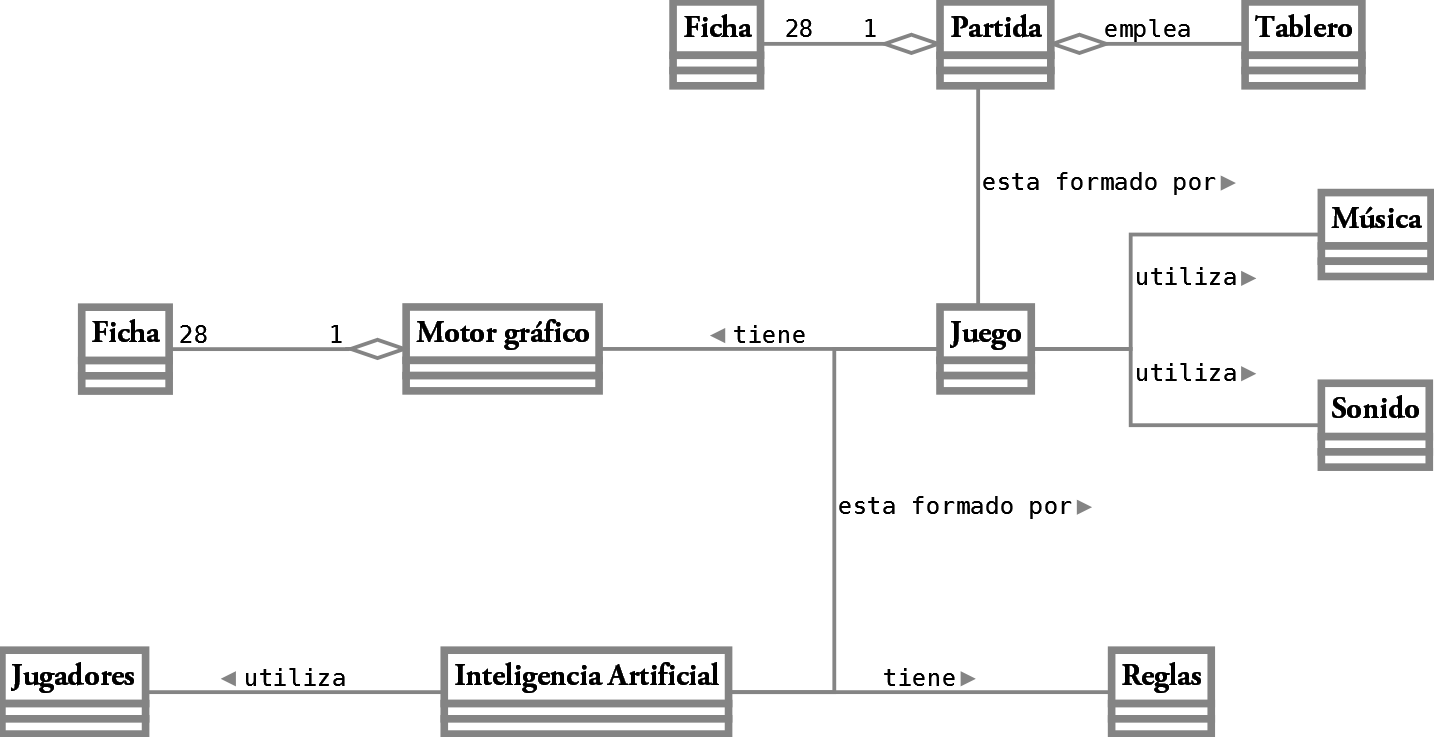
\includegraphics[scale=0.18]{diagrama_clases.png}
  \end{center}
  \caption{Diagrama de clases para los requisitos obtenidos}
\end{figure}


\subsection{Modelo de comportamiento del sistema}

El modelo de comportamiento define cómo debe actuar un sistema; este sistema a considerar es el que
engloba a todos los objetos, y el modelo consta de dos partes:
\begin{itemize}
    \item El Diagrama de secuencias del sistema el cual muestra la secuencia de eventos entre los actores
        y el sistema.
    \item Los Contrato de las operaciones del sistema que describen el efecto que producen las operaciones
        del sistema.
\end{itemize}

\subsubsection{Modelo de comportamiento partida simple}

\begin{figure}[h]
  \label{diagrama_clases}
  \begin{center}
    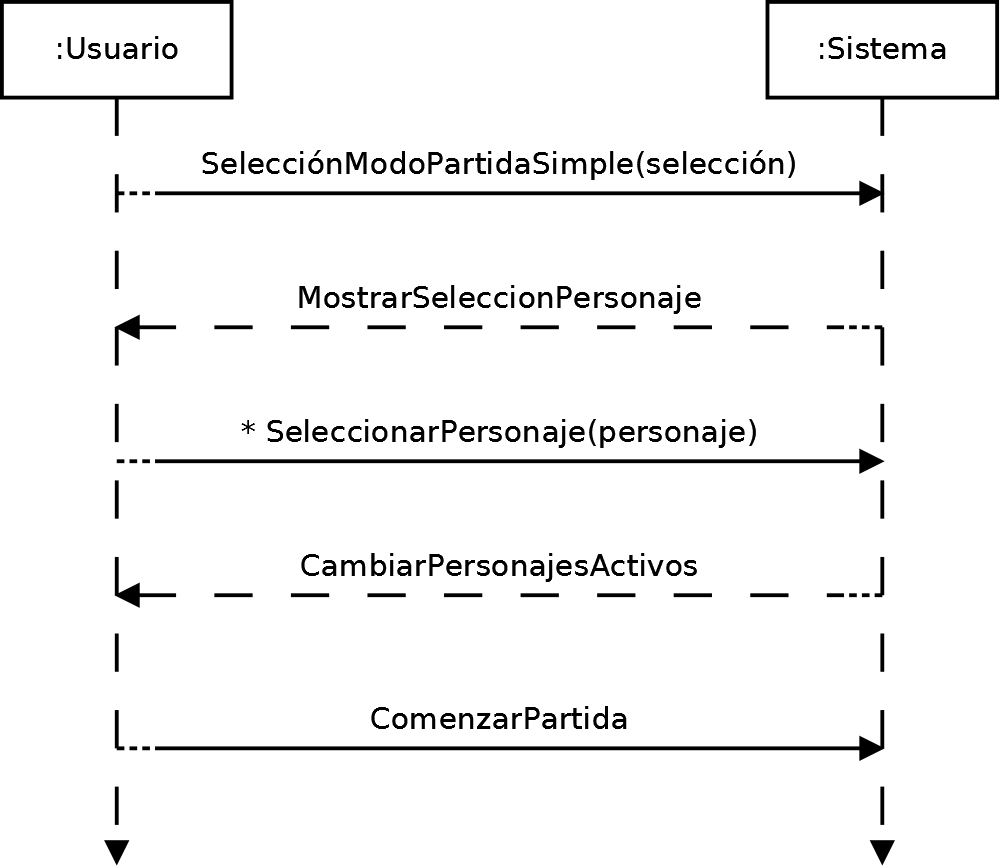
\includegraphics[scale=0.15]{diagrama_clases_partida.png}
  \end{center}
  \caption{Diagrama de secuencia para el caso de uso Partida simple}
\end{figure}

\textbf{Contrato de operaciones}
\begin{description}
    \item[Operación] Menú principal
    \item[Actores] Usuario, sistema 
    \item[Responsabilidades] Seleccionar los personajes que intervendrán en la partida actual
    \item[Precondiciones] Ninguna
    \item[Postcondiciones] Selección de personajes para la partida, comienzo de partida
\end{description}
